In this note we list all congruence lattices of transitive G-sets in $\Eq(n)$
for $n=3,\dots, 15$ (with a few for $n=16$ as well).  This is possible because
of the following observation: If $G$ is an arbitrary transitive permutation
group of degree $n$ (the number of moved points), then the index of the
stabilizer $G_x$ is $[G: G_x] = n$, and the transitive G-set $\<X; G\> \cong 
\<G/G_x; G\>$ has $|X|=n$ and congruence lattice $\Con\<X; G\> \leq \Eq(n)$,
which is isomorphic to the interval $[G_x, G]$ in the subgroup lattice of $G$.  
Thus, sublattices of $\Eq(n)$ which are congruence lattices of transitive G-sets
are the intervals above stabilizer subgroups of transitive groups of degree $n$.
\\[8pt]
GAP has a library of transitive permutation groups of degree at most 30.
Therefore, for a transitive G-set $\<X; G\>$ with $|X|\leq 30$, the shape of $\Con\<X;
G\>$ can be computed with three simple GAP commands.  Take, for example,
$G=$ {\tt TransitiveGroup(4,2)} (the second transitive group of
degree 4).  The covering relations of the sublattice $\Con\<X; G\> \leq \Eq(4)$
are found by
{\small
\begin{verbatim}
gap> G := TransitiveGroup(4,2);     % returns E(4) = 2[x]2
gap> H := Stabilizer(G,1);          % returns Group(())
gap> intHG := IntermediateSubgroups(G,H);
rec( subgroups := [ Group([ (1,2)(3,4) ]), Group([ (1,4)(2,3) ]), Group([ (1,3)(2,4) ]) ], 
  inclusions := [ [ 0, 1 ], [ 0, 2 ], [ 0, 3 ], [ 1, 4 ], [ 2, 4 ], [ 3, 4 ] ] )
\end{verbatim}}
\noindent The list {\tt intHG.inclusions} (the last line above) shows that $\Con\<X; G\> \cong M_3$.
\\[6pt]
The following displays the number of transitive permutation groups of degree at
most 20: 
{\small
\begin{verbatim}
gap> List([1..20], x->NrTransitiveGroups(x));
[ 1, 1, 2, 5, 5, 16, 7, 50, 34, 45, 8, 301, 9, 63, 104, 1954, 10, 983, 8, 1117 ]
\end{verbatim}}
\noindent Many of these groups are \emph{primitive}, that is, the congruence
lattice of the associated G-set is just the two element lattice.  For example,
all transitive groups of prime degree are primitive.  So, in the list below, we
only present those G-set congruence lattices in $\Eq(n)$ for $n=4, 6, 8, 9,
10, 12, 14, 15$. 

Properties of transitive groups a given degree, $n$, can be checked with
the {\tt AllTransitiveGroups} function with {\tt NrMovedPoints} parameter set to
$n$.  For example, we can check for primitivity of transitive groups of degrees
5, 6, 7, and 11 as follows:
{\small
\begin{verbatim}
gap> List(AllTransitiveGroups(NrMovedPoints,5),IsPrimitive);
[ true, true, true, true, true ]
gap> List(AllTransitiveGroups(NrMovedPoints,6),IsPrimitive);
[ false, false, false, false, false, false, false, false, false, false, false, true,...
  ... false, true, true, true ]
gap> List(AllTransitiveGroups(NrMovedPoints,7),IsPrimitive);
[ true, true, true, true, true, true, true ]
gap> List(AllTransitiveGroups(NrMovedPoints,11),IsPrimitive);
[ true, true, true, true, true, true, true, true ]
\end{verbatim}}

%% \input{TransitiveGsetCongEx4.tex}
\begin{figure}[h]
\caption{Transitive G-set congruence lattices in Eq(4)}
\label{fig:4}
\begin{center}
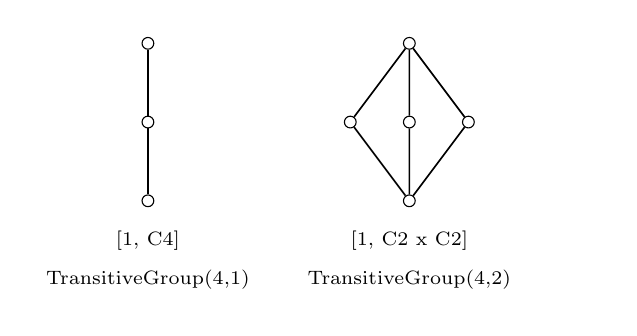
\begin{tikzpicture}[scale=.5]
\matrix[column sep=5mm,row sep=5mm]
{
\node (0) at (0,0) [draw, circle,inner sep=1.5pt] {};
\node (1) at (-0,1) [draw, circle, inner sep=1.5pt] {};
\node (2) at (-0,2) [draw, circle, inner sep=1.5pt] {};
\draw[font=\scriptsize] (0,-.5) node {[1, C4]};
\draw[font=\scriptsize] (0,-1) node {TransitiveGroup(4,1) };

\draw[semithick]
(0) to (1)
(1) to (2);
&
\node (0) at (0,0) [draw, circle,inner sep=1.5pt] {};
\node (1) at (-0,1) [draw, circle, inner sep=1.5pt] {};
\node (2) at (0.75,1) [draw, circle, inner sep=1.5pt] {};
\node (3) at (-0.75,1) [draw, circle, inner sep=1.5pt] {};
\node (4) at (-0,2) [draw, circle, inner sep=1.5pt] {};
\draw[font=\scriptsize] (0,-.5) node {[1, C2 x C2]};
\draw[font=\scriptsize] (0,-1) node {TransitiveGroup(4,2) };

\draw[semithick]
(0) to (1)
(0) to (2)
(0) to (3)
(1) to (4)
(2) to (4)
(3) to (4);
&
& \\
};
\end{tikzpicture}
\end{center}
\end{figure}



%% \input{TransitiveGsetCongEx6.tex}
\begin{figure}[h]
\caption{Transitive G-set congruence lattices in Eq(6)}
\label{fig:6}
\begin{center}
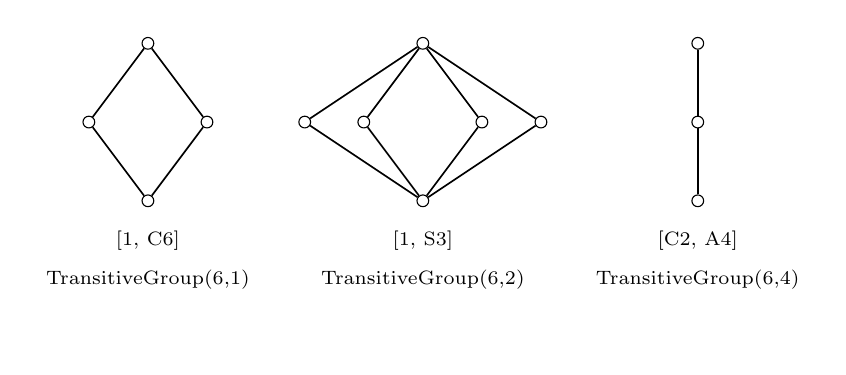
\begin{tikzpicture}[scale=.5]
\matrix[column sep=5mm,row sep=5mm]
{
\node (0) at (0,0) [draw, circle,inner sep=1.5pt] {};
\node (1) at (0.75,1) [draw, circle, inner sep=1.5pt] {};
\node (2) at (-0.75,1) [draw, circle, inner sep=1.5pt] {};
\node (3) at (-0,2) [draw, circle, inner sep=1.5pt] {};
\draw[font=\scriptsize] (0,-.5) node {[1, C6]};
\draw[font=\scriptsize] (0,-1) node {TransitiveGroup(6,1) };

\draw[semithick]
(0) to (1)
(0) to (2)
(1) to (3)
(2) to (3);
&
\node (0) at (0,0) [draw, circle,inner sep=1.5pt] {};
\node (1) at (0.75,1) [draw, circle, inner sep=1.5pt] {};
\node (2) at (-0.75,1) [draw, circle, inner sep=1.5pt] {};
\node (3) at (1.5,1) [draw, circle, inner sep=1.5pt] {};
\node (4) at (-1.5,1) [draw, circle, inner sep=1.5pt] {};
\node (5) at (-0,2) [draw, circle, inner sep=1.5pt] {};
\draw[font=\scriptsize] (0,-.5) node {[1, S3]};
\draw[font=\scriptsize] (0,-1) node {TransitiveGroup(6,2) };

\draw[semithick]
(0) to (1)
(0) to (2)
(0) to (3)
(0) to (4)
(1) to (5)
(2) to (5)
(3) to (5)
(4) to (5);
&
\node (0) at (0,0) [draw, circle,inner sep=1.5pt] {};
\node (1) at (-0,1) [draw, circle, inner sep=1.5pt] {};
\node (2) at (-0,2) [draw, circle, inner sep=1.5pt] {};
\draw[font=\scriptsize] (0,-.5) node {[C2, A4]};
\draw[font=\scriptsize] (0,-1) node {TransitiveGroup(6,4) };

\draw[semithick]
(0) to (1)
(1) to (2);
\\
\\
};
\end{tikzpicture}
\end{center}
\end{figure}

\newpage


%\input{TransitiveGsetCongEx8.tex}
\begin{figure}[h]
\caption{Transitive G-set congruence lattices in Eq(8)}
\label{fig:8}
\begin{center}
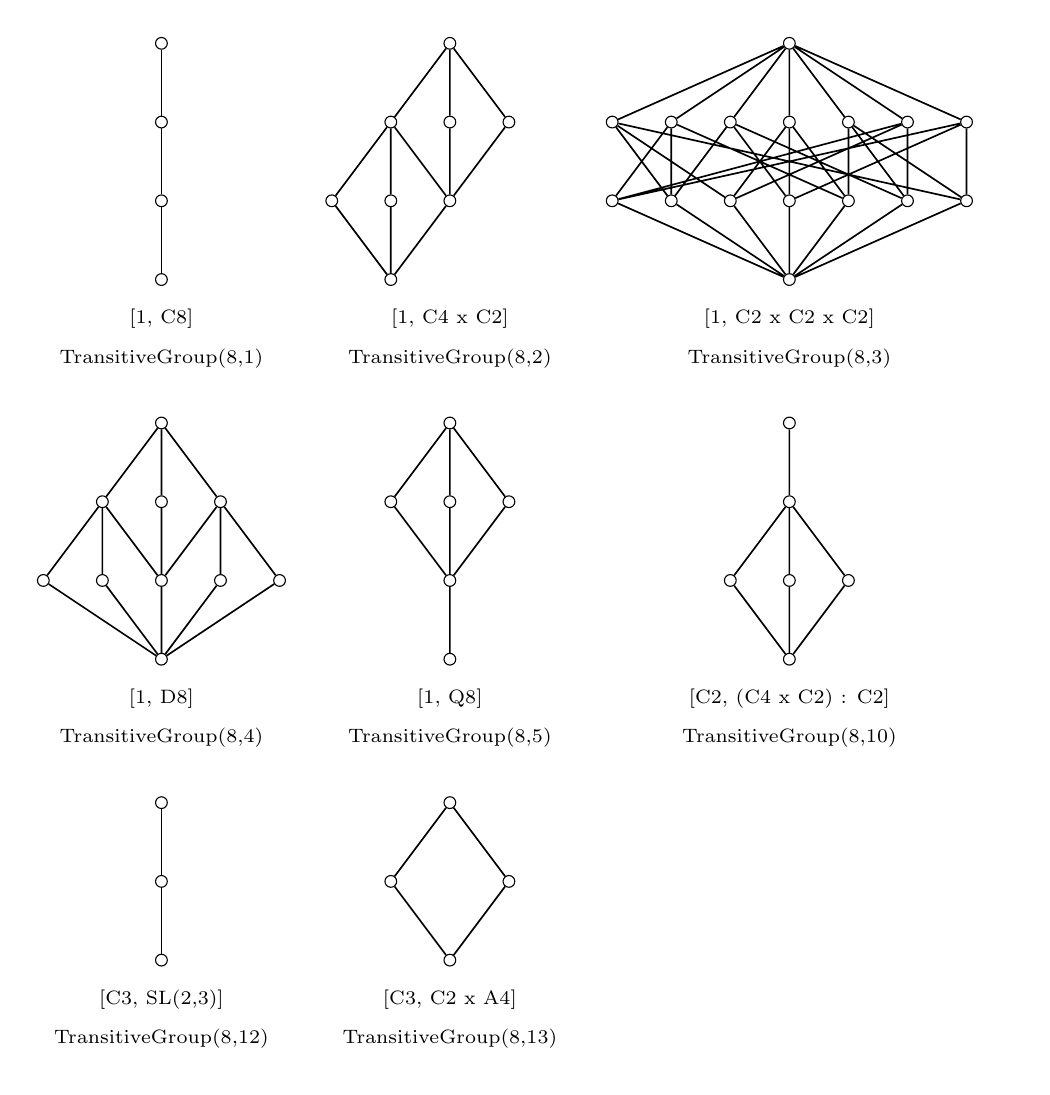
\begin{tikzpicture}[scale=.5]
\matrix[column sep=5mm,row sep=5mm]
{
\node (0) at (0,0) [draw, circle,inner sep=1.5pt] {};
\node (1) at (-0,1) [draw, circle, inner sep=1.5pt] {};
\node (2) at (-0,2) [draw, circle, inner sep=1.5pt] {};
\node (3) at (-0,3) [draw, circle, inner sep=1.5pt] {};
\draw[font=\scriptsize] (0,-.5) node {[1, C8]};
\draw[font=\scriptsize] (0,-1) node {TransitiveGroup(8,1) };

\draw[semithick]
(0) to (1)
(1) to (2)
(2) to (3);
&
%\node (0) at (0,0) [draw, circle,inner sep=1.5pt] {};
\node (0) at (-0.75,0) [draw, circle,inner sep=1.5pt] {};
\node (1) at (-0,1) [draw, circle, inner sep=1.5pt] {};
%\node (2) at (0.75,1) [draw, circle, inner sep=1.5pt] {};
\node (2) at (-1.5,1) [draw, circle, inner sep=1.5pt] {};
\node (3) at (-0.75,1) [draw, circle, inner sep=1.5pt] {};
%\node (4) at (-0,2) [draw, circle, inner sep=1.5pt] {};
\node (4) at (-0.75,2) [draw, circle, inner sep=1.5pt] {};
\node (5) at (0.75,2) [draw, circle, inner sep=1.5pt] {};
%\node (6) at (-0.75,2) [draw, circle, inner sep=1.5pt] {};
\node (6) at (0,2) [draw, circle, inner sep=1.5pt] {};
\node (7) at (-0,3) [draw, circle, inner sep=1.5pt] {};
\draw[font=\scriptsize] (0,-.5) node {[1, C4 x C2]};
\draw[font=\scriptsize] (0,-1) node {TransitiveGroup(8,2) };

\draw[semithick]
(0) to (1)
(0) to (2)
(0) to (3)
(1) to (4)
(1) to (5)
(1) to (6)
(2) to (4)
(3) to (4)
(4) to (7)
(5) to (7)
(6) to (7);
&
\node (0) at (0,0) [draw, circle,inner sep=1.5pt] {};
\node (1) at (-0,1) [draw, circle, inner sep=1.5pt] {};
\node (2) at (0.75,1) [draw, circle, inner sep=1.5pt] {};
\node (3) at (-0.75,1) [draw, circle, inner sep=1.5pt] {};
\node (4) at (1.5,1) [draw, circle, inner sep=1.5pt] {};
\node (5) at (-1.5,1) [draw, circle, inner sep=1.5pt] {};
\node (6) at (2.25,1) [draw, circle, inner sep=1.5pt] {};
\node (7) at (-2.25,1) [draw, circle, inner sep=1.5pt] {};
\node (8) at (-0,2) [draw, circle, inner sep=1.5pt] {};
\node (9) at (0.75,2) [draw, circle, inner sep=1.5pt] {};
\node (10) at (-0.75,2) [draw, circle, inner sep=1.5pt] {};
\node (11) at (1.5,2) [draw, circle, inner sep=1.5pt] {};
\node (12) at (-1.5,2) [draw, circle, inner sep=1.5pt] {};
\node (13) at (2.25,2) [draw, circle, inner sep=1.5pt] {};
\node (14) at (-2.25,2) [draw, circle, inner sep=1.5pt] {};
\node (15) at (-0,3) [draw, circle, inner sep=1.5pt] {};
\draw[font=\scriptsize] (0,-.5) node {[1, C2 x C2 x C2]};
\draw[font=\scriptsize] (0,-1) node {TransitiveGroup(8,3) };

\draw[semithick]
(0) to (1)
(0) to (2)
(0) to (3)
(0) to (4)
(0) to (5)
(0) to (6)
(0) to (7)
(1) to (8)
(1) to (10)
(1) to (13)
(2) to (8)
(2) to (9)
(2) to (12)
(3) to (8)
(3) to (11)
(3) to (14)
(4) to (9)
(4) to (10)
(4) to (11)
(5) to (10)
(5) to (12)
(5) to (14)
(6) to (9)
(6) to (13)
(6) to (14)
(7) to (11)
(7) to (12)
(7) to (13)
(8) to (15)
(9) to (15)
(10) to (15)
(11) to (15)
(12) to (15)
(13) to (15)
(14) to (15);
\\
\node (0) at (0,0) [draw, circle,inner sep=1.5pt] {};
\node (1) at (-0,1) [draw, circle, inner sep=1.5pt] {};
\node (2) at (0.75,1) [draw, circle, inner sep=1.5pt] {};
% \node (3) at (-0.75,1) [draw, circle, inner sep=1.5pt] {};
% \node (4) at (1.5,1) [draw, circle, inner sep=1.5pt] {};
\node (3) at (1.5,1) [draw, circle, inner sep=1.5pt] {};
\node (4) at (-0.75,1) [draw, circle, inner sep=1.5pt] {};
\node (5) at (-1.5,1) [draw, circle, inner sep=1.5pt] {};
% \node (6) at (-0,2) [draw, circle, inner sep=1.5pt] {};
% \node (7) at (0.75,2) [draw, circle, inner sep=1.5pt] {};
\node (6) at (0.75,2) [draw, circle, inner sep=1.5pt] {};
\node (7) at (0,2) [draw, circle, inner sep=1.5pt] {};
\node (8) at (-0.75,2) [draw, circle, inner sep=1.5pt] {};
\node (9) at (-0,3) [draw, circle, inner sep=1.5pt] {};
\draw[font=\scriptsize] (0,-.5) node {[1, D8]};
\draw[font=\scriptsize] (0,-1) node {TransitiveGroup(8,4) };

\draw[semithick]
(0) to (1)
(0) to (2)
(0) to (3)
(0) to (4)
(0) to (5)
(1) to (6)
(1) to (7)
(1) to (8)
(2) to (6)
(3) to (6)
(4) to (8)
(5) to (8)
(6) to (9)
(7) to (9)
(8) to (9);
&
\node (0) at (0,0) [draw, circle,inner sep=1.5pt] {};
\node (1) at (-0,1) [draw, circle, inner sep=1.5pt] {};
\node (2) at (-0,2) [draw, circle, inner sep=1.5pt] {};
\node (3) at (0.75,2) [draw, circle, inner sep=1.5pt] {};
\node (4) at (-0.75,2) [draw, circle, inner sep=1.5pt] {};
\node (5) at (-0,3) [draw, circle, inner sep=1.5pt] {};
\draw[font=\scriptsize] (0,-.5) node {[1, Q8]};
\draw[font=\scriptsize] (0,-1) node {TransitiveGroup(8,5) };

\draw[semithick]
(0) to (1)
(1) to (2)
(1) to (3)
(1) to (4)
(2) to (5)
(3) to (5)
(4) to (5);
&
\node (0) at (0,0) [draw, circle,inner sep=1.5pt] {};
\node (1) at (-0,1) [draw, circle, inner sep=1.5pt] {};
\node (2) at (0.75,1) [draw, circle, inner sep=1.5pt] {};
\node (3) at (-0.75,1) [draw, circle, inner sep=1.5pt] {};
\node (4) at (-0,2) [draw, circle, inner sep=1.5pt] {};
\node (5) at (-0,3) [draw, circle, inner sep=1.5pt] {};
\draw[font=\scriptsize] (0,-.5) node {[C2, (C4 x C2) : C2]};
\draw[font=\scriptsize] (0,-1) node {TransitiveGroup(8,10) };

\draw[semithick]
(0) to (1)
(0) to (2)
(0) to (3)
(1) to (4)
(2) to (4)
(3) to (4)
(4) to (5);
\\
\node (0) at (0,0) [draw, circle,inner sep=1.5pt] {};
\node (1) at (-0,1) [draw, circle, inner sep=1.5pt] {};
\node (2) at (-0,2) [draw, circle, inner sep=1.5pt] {};
\draw[font=\scriptsize] (0,-.5) node {[C3, SL(2,3)]};
\draw[font=\scriptsize] (0,-1) node {TransitiveGroup(8,12) };

\draw[semithick]
(0) to (1)
(1) to (2);
&
\node (0) at (0,0) [draw, circle,inner sep=1.5pt] {};
\node (1) at (0.75,1) [draw, circle, inner sep=1.5pt] {};
\node (2) at (-0.75,1) [draw, circle, inner sep=1.5pt] {};
\node (3) at (-0,2) [draw, circle, inner sep=1.5pt] {};
\draw[font=\scriptsize] (0,-.5) node {[C3, C2 x A4]};
\draw[font=\scriptsize] (0,-1) node {TransitiveGroup(8,13) };

\draw[semithick]
(0) to (1)
(0) to (2)
(1) to (3)
(2) to (3);
&
& \\
};
\end{tikzpicture}
\end{center}
\end{figure}

\newpage

%% \input{TransitiveGsetCongEx9.tex}
\begin{figure}[h]
\caption{Transitive G-set congruence lattices in Eq(9)}
\label{fig:9}
\begin{center}
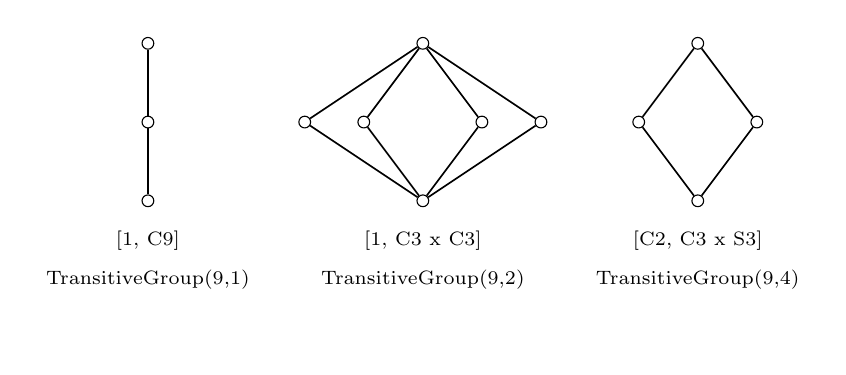
\begin{tikzpicture}[scale=.5]
\matrix[column sep=5mm,row sep=5mm]
{
\node (0) at (0,0) [draw, circle,inner sep=1.5pt] {};
\node (1) at (-0,1) [draw, circle, inner sep=1.5pt] {};
\node (2) at (-0,2) [draw, circle, inner sep=1.5pt] {};
\draw[font=\scriptsize] (0,-.5) node {[1, C9]};
\draw[font=\scriptsize] (0,-1) node {TransitiveGroup(9,1) };

\draw[semithick]
(0) to (1)
(1) to (2);
&
\node (0) at (0,0) [draw, circle,inner sep=1.5pt] {};
\node (1) at (0.75,1) [draw, circle, inner sep=1.5pt] {};
\node (2) at (-0.75,1) [draw, circle, inner sep=1.5pt] {};
\node (3) at (1.5,1) [draw, circle, inner sep=1.5pt] {};
\node (4) at (-1.5,1) [draw, circle, inner sep=1.5pt] {};
\node (5) at (-0,2) [draw, circle, inner sep=1.5pt] {};
\draw[font=\scriptsize] (0,-.5) node {[1, C3 x C3]};
\draw[font=\scriptsize] (0,-1) node {TransitiveGroup(9,2) };

\draw[semithick]
(0) to (1)
(0) to (2)
(0) to (3)
(0) to (4)
(1) to (5)
(2) to (5)
(3) to (5)
(4) to (5);
&
\node (0) at (0,0) [draw, circle,inner sep=1.5pt] {};
\node (1) at (0.75,1) [draw, circle, inner sep=1.5pt] {};
\node (2) at (-0.75,1) [draw, circle, inner sep=1.5pt] {};
\node (3) at (-0,2) [draw, circle, inner sep=1.5pt] {};
\draw[font=\scriptsize] (0,-.5) node {[C2, C3 x S3]};
\draw[font=\scriptsize] (0,-1) node {TransitiveGroup(9,4) };

\draw[semithick]
(0) to (1)
(0) to (2)
(1) to (3)
(2) to (3);
\\
\\
};
\end{tikzpicture}
\end{center}
\end{figure}

\newpage





%% \input{TransitiveGsetCongEx10.tex}
\begin{figure}[h]
\caption{Transitive G-set congruence lattices in Eq(10)}
\label{fig:10}
\begin{center}
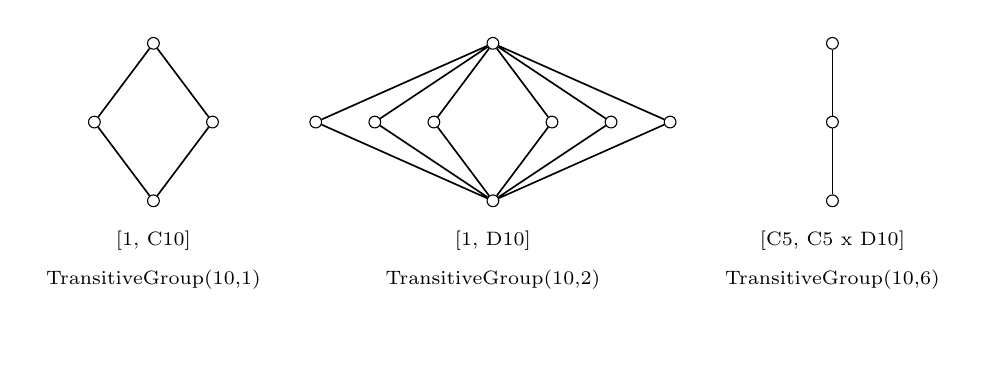
\begin{tikzpicture}[scale=.5]
\matrix[column sep=5mm,row sep=5mm]
{
\node (0) at (0,0) [draw, circle,inner sep=1.5pt] {};
\node (1) at (0.75,1) [draw, circle, inner sep=1.5pt] {};
\node (2) at (-0.75,1) [draw, circle, inner sep=1.5pt] {};
\node (3) at (-0,2) [draw, circle, inner sep=1.5pt] {};
\draw[font=\scriptsize] (0,-.5) node {[1, C10]};
\draw[font=\scriptsize] (0,-1) node {TransitiveGroup(10,1) };

\draw[semithick]
(0) to (1)
(0) to (2)
(1) to (3)
(2) to (3);
&
\node (0) at (0,0) [draw, circle,inner sep=1.5pt] {};
\node (1) at (0.75,1) [draw, circle, inner sep=1.5pt] {};
\node (2) at (-0.75,1) [draw, circle, inner sep=1.5pt] {};
\node (3) at (1.5,1) [draw, circle, inner sep=1.5pt] {};
\node (4) at (-1.5,1) [draw, circle, inner sep=1.5pt] {};
\node (5) at (2.25,1) [draw, circle, inner sep=1.5pt] {};
\node (6) at (-2.25,1) [draw, circle, inner sep=1.5pt] {};
\node (7) at (-0,2) [draw, circle, inner sep=1.5pt] {};
\draw[font=\scriptsize] (0,-.5) node {[1, D10]};
\draw[font=\scriptsize] (0,-1) node {TransitiveGroup(10,2) };

\draw[semithick]
(0) to (1)
(0) to (2)
(0) to (3)
(0) to (4)
(0) to (5)
(0) to (6)
(1) to (7)
(2) to (7)
(3) to (7)
(4) to (7)
(5) to (7)
(6) to (7);
&
\node (0) at (0,0) [draw, circle,inner sep=1.5pt] {};
\node (1) at (-0,1) [draw, circle, inner sep=1.5pt] {};
\node (2) at (-0,2) [draw, circle, inner sep=1.5pt] {};
\draw[font=\scriptsize] (0,-.5) node {[C5, C5 x D10]};
\draw[font=\scriptsize] (0,-1) node {TransitiveGroup(10,6) };

\draw[semithick]
(0) to (1)
(1) to (2);
\\
\\
};
\end{tikzpicture}
\end{center}
\end{figure}

\newpage


%% \input{TransitiveGsetCongEx12.tex}
\begin{figure}[h]
\caption{Transitive G-set congruence lattices in Eq(12)}
\label{fig:12}
\begin{center}
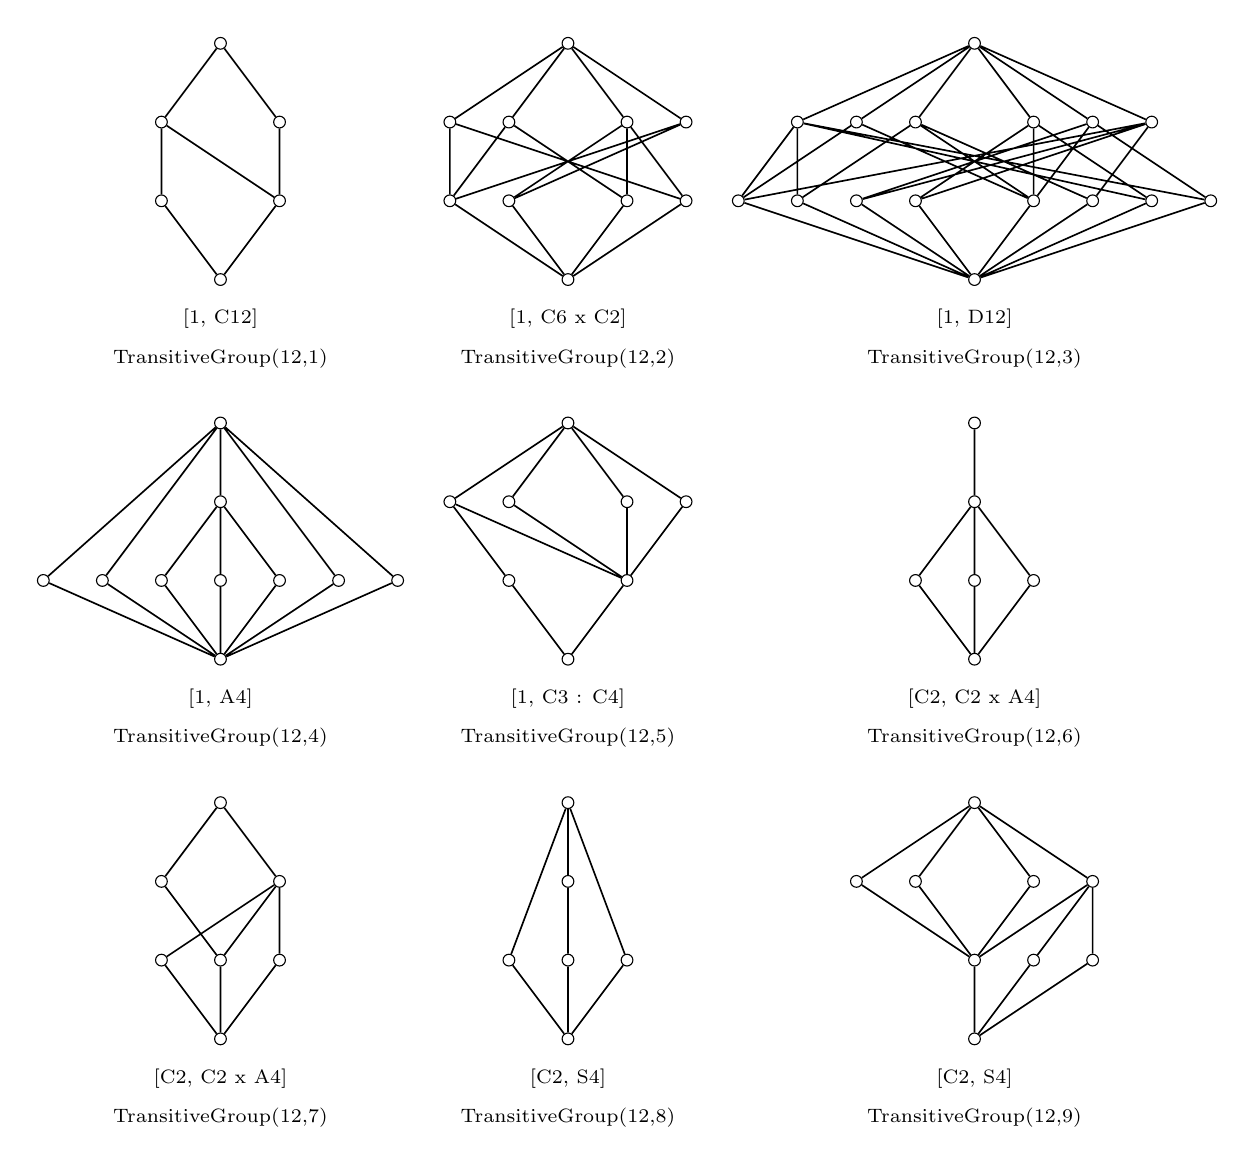
\begin{tikzpicture}[scale=.5]
\matrix[column sep=5mm,row sep=5mm]
{
\node (0) at (0,0) [draw, circle,inner sep=1.5pt] {};
\node (1) at (0.75,1) [draw, circle, inner sep=1.5pt] {};
\node (2) at (-0.75,1) [draw, circle, inner sep=1.5pt] {};
\node (3) at (0.75,2) [draw, circle, inner sep=1.5pt] {};
\node (4) at (-0.75,2) [draw, circle, inner sep=1.5pt] {};
\node (5) at (-0,3) [draw, circle, inner sep=1.5pt] {};
\draw[font=\scriptsize] (0,-.5) node {[1, C12]};
\draw[font=\scriptsize] (0,-1) node {TransitiveGroup(12,1) };

\draw[semithick]
(0) to (1)
(0) to (2)
(1) to (3)
(1) to (4)
(2) to (4)
(3) to (5)
(4) to (5);
&
\node (0) at (0,0) [draw, circle,inner sep=1.5pt] {};
\node (1) at (0.75,1) [draw, circle, inner sep=1.5pt] {};
\node (2) at (-0.75,1) [draw, circle, inner sep=1.5pt] {};
\node (3) at (1.5,1) [draw, circle, inner sep=1.5pt] {};
\node (4) at (-1.5,1) [draw, circle, inner sep=1.5pt] {};
\node (5) at (0.75,2) [draw, circle, inner sep=1.5pt] {};
\node (6) at (-0.75,2) [draw, circle, inner sep=1.5pt] {};
\node (7) at (1.5,2) [draw, circle, inner sep=1.5pt] {};
\node (8) at (-1.5,2) [draw, circle, inner sep=1.5pt] {};
\node (9) at (-0,3) [draw, circle, inner sep=1.5pt] {};
\draw[font=\scriptsize] (0,-.5) node {[1, C6 x C2]};
\draw[font=\scriptsize] (0,-1) node {TransitiveGroup(12,2) };

\draw[semithick]
(0) to (1)
(0) to (2)
(0) to (3)
(0) to (4)
(1) to (5)
(1) to (6)
(2) to (5)
(2) to (7)
(3) to (5)
(3) to (8)
(4) to (6)
(4) to (7)
(4) to (8)
(5) to (9)
(6) to (9)
(7) to (9)
(8) to (9);
&
\node (0) at (0,0) [draw, circle,inner sep=1.5pt] {};
\node (1) at (0.75,1) [draw, circle, inner sep=1.5pt] {};
\node (2) at (-0.75,1) [draw, circle, inner sep=1.5pt] {};
\node (3) at (1.5,1) [draw, circle, inner sep=1.5pt] {};
\node (4) at (-1.5,1) [draw, circle, inner sep=1.5pt] {};
\node (5) at (2.25,1) [draw, circle, inner sep=1.5pt] {};
\node (6) at (-2.25,1) [draw, circle, inner sep=1.5pt] {};
\node (7) at (3,1) [draw, circle, inner sep=1.5pt] {};
\node (8) at (-3,1) [draw, circle, inner sep=1.5pt] {};
\node (9) at (0.75,2) [draw, circle, inner sep=1.5pt] {};
\node (10) at (-0.75,2) [draw, circle, inner sep=1.5pt] {};
\node (11) at (1.5,2) [draw, circle, inner sep=1.5pt] {};
\node (12) at (-1.5,2) [draw, circle, inner sep=1.5pt] {};
\node (13) at (2.25,2) [draw, circle, inner sep=1.5pt] {};
\node (14) at (-2.25,2) [draw, circle, inner sep=1.5pt] {};
\node (15) at (-0,3) [draw, circle, inner sep=1.5pt] {};
\draw[font=\scriptsize] (0,-.5) node {[1, D12]};
\draw[font=\scriptsize] (0,-1) node {TransitiveGroup(12,3) };

\draw[semithick]
(0) to (1)
(0) to (2)
(0) to (3)
(0) to (4)
(0) to (5)
(0) to (6)
(0) to (7)
(0) to (8)
(1) to (9)
(1) to (10)
(1) to (11)
(1) to (12)
(2) to (9)
(2) to (13)
(3) to (10)
(3) to (13)
(4) to (11)
(4) to (13)
(5) to (9)
(5) to (14)
(6) to (10)
(6) to (14)
(7) to (11)
(7) to (14)
(8) to (12)
(8) to (13)
(8) to (14)
(9) to (15)
(10) to (15)
(11) to (15)
(12) to (15)
(13) to (15)
(14) to (15);
\\
\node (0) at (0,0) [draw, circle,inner sep=1.5pt] {};
\node (1) at (-0,1) [draw, circle, inner sep=1.5pt] {};
\node (2) at (0.75,1) [draw, circle, inner sep=1.5pt] {};
\node (3) at (-0.75,1) [draw, circle, inner sep=1.5pt] {};
\node (4) at (1.5,1) [draw, circle, inner sep=1.5pt] {};
\node (5) at (-1.5,1) [draw, circle, inner sep=1.5pt] {};
\node (6) at (2.25,1) [draw, circle, inner sep=1.5pt] {};
\node (7) at (-2.25,1) [draw, circle, inner sep=1.5pt] {};
\node (8) at (-0,2) [draw, circle, inner sep=1.5pt] {};
\node (9) at (-0,3) [draw, circle, inner sep=1.5pt] {};
\draw[font=\scriptsize] (0,-.5) node {[1, A4]};
\draw[font=\scriptsize] (0,-1) node {TransitiveGroup(12,4) };

\draw[semithick]
(0) to (1)
(0) to (2)
(0) to (3)
(0) to (4)
(0) to (5)
(0) to (6)
(0) to (7)
(1) to (8)
(2) to (8)
(3) to (8)
(4) to (9)
(5) to (9)
(6) to (9)
(7) to (9)
(8) to (9);
&
\node (0) at (0,0) [draw, circle,inner sep=1.5pt] {};
\node (1) at (0.75,1) [draw, circle, inner sep=1.5pt] {};
\node (2) at (-0.75,1) [draw, circle, inner sep=1.5pt] {};
\node (3) at (0.75,2) [draw, circle, inner sep=1.5pt] {};
\node (4) at (-0.75,2) [draw, circle, inner sep=1.5pt] {};
\node (5) at (1.5,2) [draw, circle, inner sep=1.5pt] {};
\node (6) at (-1.5,2) [draw, circle, inner sep=1.5pt] {};
\node (7) at (-0,3) [draw, circle, inner sep=1.5pt] {};
\draw[font=\scriptsize] (0,-.5) node {[1, C3 : C4]};
\draw[font=\scriptsize] (0,-1) node {TransitiveGroup(12,5) };

\draw[semithick]
(0) to (1)
(0) to (2)
(1) to (3)
(1) to (4)
(1) to (5)
(1) to (6)
(2) to (6)
(3) to (7)
(4) to (7)
(5) to (7)
(6) to (7);
&
\node (0) at (0,0) [draw, circle,inner sep=1.5pt] {};
\node (1) at (-0,1) [draw, circle, inner sep=1.5pt] {};
\node (2) at (0.75,1) [draw, circle, inner sep=1.5pt] {};
\node (3) at (-0.75,1) [draw, circle, inner sep=1.5pt] {};
\node (4) at (-0,2) [draw, circle, inner sep=1.5pt] {};
\node (5) at (-0,3) [draw, circle, inner sep=1.5pt] {};
\draw[font=\scriptsize] (0,-.5) node {[C2, C2 x A4]};
\draw[font=\scriptsize] (0,-1) node {TransitiveGroup(12,6) };

\draw[semithick]
(0) to (1)
(0) to (2)
(0) to (3)
(1) to (4)
(2) to (4)
(3) to (4)
(4) to (5);
\\
\node (0) at (0,0) [draw, circle,inner sep=1.5pt] {};
\node (1) at (-0,1) [draw, circle, inner sep=1.5pt] {};
\node (2) at (0.75,1) [draw, circle, inner sep=1.5pt] {};
\node (3) at (-0.75,1) [draw, circle, inner sep=1.5pt] {};
\node (4) at (0.75,2) [draw, circle, inner sep=1.5pt] {};
\node (5) at (-0.75,2) [draw, circle, inner sep=1.5pt] {};
\node (6) at (-0,3) [draw, circle, inner sep=1.5pt] {};
\draw[font=\scriptsize] (0,-.5) node {[C2, C2 x A4]};
\draw[font=\scriptsize] (0,-1) node {TransitiveGroup(12,7) };

\draw[semithick]
(0) to (1)
(0) to (2)
(0) to (3)
(1) to (4)
(1) to (5)
(2) to (4)
(3) to (4)
(4) to (6)
(5) to (6);
&
\node (0) at (0,0) [draw, circle,inner sep=1.5pt] {};
\node (1) at (-0,1) [draw, circle, inner sep=1.5pt] {};
\node (2) at (0.75,1) [draw, circle, inner sep=1.5pt] {};
\node (3) at (-0.75,1) [draw, circle, inner sep=1.5pt] {};
\node (4) at (-0,2) [draw, circle, inner sep=1.5pt] {};
\node (5) at (-0,3) [draw, circle, inner sep=1.5pt] {};
\draw[font=\scriptsize] (0,-.5) node {[C2, S4]};
\draw[font=\scriptsize] (0,-1) node {TransitiveGroup(12,8) };

\draw[semithick]
(0) to (1)
(0) to (2)
(0) to (3)
(1) to (4)
(2) to (5)
(3) to (5)
(4) to (5);
&
 \node (0) at (0,0) [draw, circle,inner sep=1.5pt] {};
% \node (1) at (-0,1) [draw, circle, inner sep=1.5pt] {};
% \node (2) at (0.75,1) [draw, circle, inner sep=1.5pt] {};
% \node (3) at (-0.75,1) [draw, circle, inner sep=1.5pt] {};
%\node (0) at (0.75,0) [draw, circle,inner sep=1.5pt] {};
\node (1) at (0.75,1) [draw, circle, inner sep=1.5pt] {};
\node (2) at (1.5,1) [draw, circle, inner sep=1.5pt] {};
\node (3) at (0,1) [draw, circle, inner sep=1.5pt] {};
\node (4) at (0.75,2) [draw, circle, inner sep=1.5pt] {};
\node (5) at (-0.75,2) [draw, circle, inner sep=1.5pt] {};
\node (6) at (1.5,2) [draw, circle, inner sep=1.5pt] {};
\node (7) at (-1.5,2) [draw, circle, inner sep=1.5pt] {};
\node (8) at (-0,3) [draw, circle, inner sep=1.5pt] {};
\draw[font=\scriptsize] (0,-.5) node {[C2, S4]};
\draw[font=\scriptsize] (0,-1) node {TransitiveGroup(12,9) };

\draw[semithick]
(0) to (1)
(0) to (2)
(0) to (3)
(1) to (6)
(2) to (6)
(3) to (4)
(3) to (5)
(3) to (6)
(3) to (7)
(4) to (8)
(5) to (8)
(6) to (8)
(7) to (8);
\\
};
\end{tikzpicture}
\end{center}
\end{figure}

\newpage

\begin{figure}[h]
\caption{Transitive G-set congruence lattices in Eq(12) (continued)}
\label{fig:12b}
\begin{center}
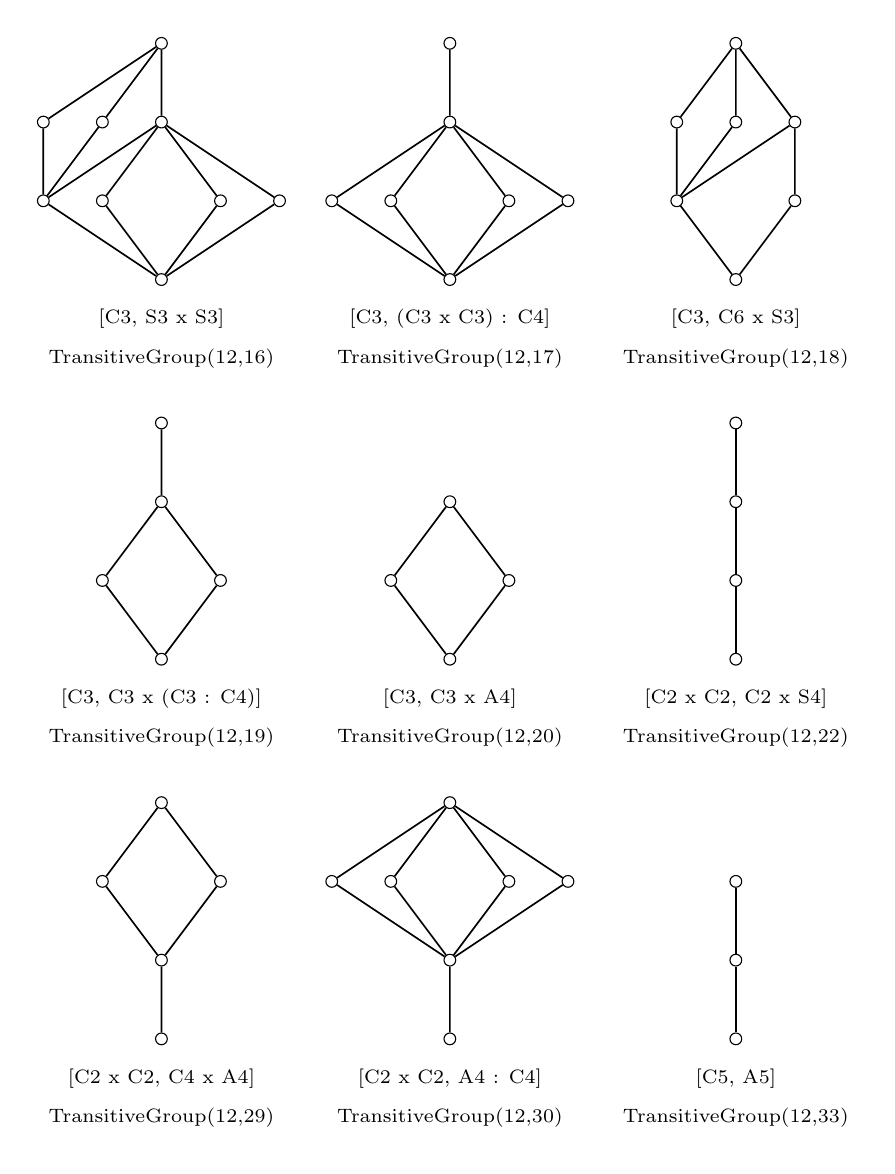
\begin{tikzpicture}[scale=.5]
\matrix[column sep=5mm,row sep=5mm]
{
\node (0) at (0,0) [draw, circle,inner sep=1.5pt] {};
\node (1) at (0.75,1) [draw, circle, inner sep=1.5pt] {};
\node (2) at (-0.75,1) [draw, circle, inner sep=1.5pt] {};
\node (3) at (1.5,1) [draw, circle, inner sep=1.5pt] {};
\node (4) at (-1.5,1) [draw, circle, inner sep=1.5pt] {};
% \node (5) at (-0,2) [draw, circle, inner sep=1.5pt] {};
% \node (6) at (0.75,2) [draw, circle, inner sep=1.5pt] {};
% \node (7) at (-0.75,2) [draw, circle, inner sep=1.5pt] {};
\node (5) at (-0.75,2) [draw, circle, inner sep=1.5pt] {};
\node (6) at (-1.5,2) [draw, circle, inner sep=1.5pt] {};
\node (7) at (0,2) [draw, circle, inner sep=1.5pt] {};
\node (8) at (-0,3) [draw, circle, inner sep=1.5pt] {};
\draw[font=\scriptsize] (0,-.5) node {[C3, S3 x S3]};
\draw[font=\scriptsize] (0,-1) node {TransitiveGroup(12,16) };

\draw[semithick]
(0) to (1)
(0) to (2)
(0) to (3)
(0) to (4)
(1) to (7)
(2) to (7)
(3) to (7)
(4) to (5)
(4) to (6)
(4) to (7)
(5) to (8)
(6) to (8)
(7) to (8);
&
\node (0) at (0,0) [draw, circle,inner sep=1.5pt] {};
\node (1) at (0.75,1) [draw, circle, inner sep=1.5pt] {};
\node (2) at (-0.75,1) [draw, circle, inner sep=1.5pt] {};
\node (3) at (1.5,1) [draw, circle, inner sep=1.5pt] {};
\node (4) at (-1.5,1) [draw, circle, inner sep=1.5pt] {};
\node (5) at (-0,2) [draw, circle, inner sep=1.5pt] {};
\node (6) at (-0,3) [draw, circle, inner sep=1.5pt] {};
\draw[font=\scriptsize] (0,-.5) node {[C3, (C3 x C3) : C4]};
\draw[font=\scriptsize] (0,-1) node {TransitiveGroup(12,17) };

\draw[semithick]
(0) to (1)
(0) to (2)
(0) to (3)
(0) to (4)
(1) to (5)
(2) to (5)
(3) to (5)
(4) to (5)
(5) to (6);
&
\node (0) at (0,0) [draw, circle,inner sep=1.5pt] {};
\node (1) at (0.75,1) [draw, circle, inner sep=1.5pt] {};
\node (2) at (-0.75,1) [draw, circle, inner sep=1.5pt] {};
\node (3) at (-0,2) [draw, circle, inner sep=1.5pt] {};
\node (4) at (0.75,2) [draw, circle, inner sep=1.5pt] {};
\node (5) at (-0.75,2) [draw, circle, inner sep=1.5pt] {};
\node (6) at (-0,3) [draw, circle, inner sep=1.5pt] {};
\draw[font=\scriptsize] (0,-.5) node {[C3, C6 x S3]};
\draw[font=\scriptsize] (0,-1) node {TransitiveGroup(12,18) };

\draw[semithick]
(0) to (1)
(0) to (2)
(1) to (4)
(2) to (3)
(2) to (4)
(2) to (5)
(3) to (6)
(4) to (6)
(5) to (6);
\\
\node (0) at (0,0) [draw, circle,inner sep=1.5pt] {};
\node (1) at (0.75,1) [draw, circle, inner sep=1.5pt] {};
\node (2) at (-0.75,1) [draw, circle, inner sep=1.5pt] {};
\node (3) at (-0,2) [draw, circle, inner sep=1.5pt] {};
\node (4) at (-0,3) [draw, circle, inner sep=1.5pt] {};
\draw[font=\scriptsize] (0,-.5) node {[C3, C3 x (C3 : C4)]};
\draw[font=\scriptsize] (0,-1) node {TransitiveGroup(12,19) };

\draw[semithick]
(0) to (1)
(0) to (2)
(1) to (3)
(2) to (3)
(3) to (4);
&
\node (0) at (0,0) [draw, circle,inner sep=1.5pt] {};
\node (1) at (0.75,1) [draw, circle, inner sep=1.5pt] {};
\node (2) at (-0.75,1) [draw, circle, inner sep=1.5pt] {};
\node (3) at (-0,2) [draw, circle, inner sep=1.5pt] {};
\draw[font=\scriptsize] (0,-.5) node {[C3, C3 x A4]};
\draw[font=\scriptsize] (0,-1) node {TransitiveGroup(12,20) };

\draw[semithick]
(0) to (1)
(0) to (2)
(1) to (3)
(2) to (3);
&
\node (0) at (0,0) [draw, circle,inner sep=1.5pt] {};
\node (1) at (-0,1) [draw, circle, inner sep=1.5pt] {};
\node (2) at (-0,2) [draw, circle, inner sep=1.5pt] {};
\node (3) at (-0,3) [draw, circle, inner sep=1.5pt] {};
\draw[font=\scriptsize] (0,-.5) node {[C2 x C2, C2 x S4]};
\draw[font=\scriptsize] (0,-1) node {TransitiveGroup(12,22) };

\draw[semithick]
(0) to (1)
(1) to (2)
(2) to (3);
\\
\node (0) at (0,0) [draw, circle,inner sep=1.5pt] {};
\node (1) at (-0,1) [draw, circle, inner sep=1.5pt] {};
\node (2) at (0.75,2) [draw, circle, inner sep=1.5pt] {};
\node (3) at (-0.75,2) [draw, circle, inner sep=1.5pt] {};
\node (4) at (-0,3) [draw, circle, inner sep=1.5pt] {};
\draw[font=\scriptsize] (0,-.5) node {[C2 x C2, C4 x A4]};
\draw[font=\scriptsize] (0,-1) node {TransitiveGroup(12,29) };

\draw[semithick]
(0) to (1)
(1) to (2)
(1) to (3)
(2) to (4)
(3) to (4);
&
\node (0) at (0,0) [draw, circle,inner sep=1.5pt] {};
\node (1) at (-0,1) [draw, circle, inner sep=1.5pt] {};
\node (2) at (0.75,2) [draw, circle, inner sep=1.5pt] {};
\node (3) at (-0.75,2) [draw, circle, inner sep=1.5pt] {};
\node (4) at (1.5,2) [draw, circle, inner sep=1.5pt] {};
\node (5) at (-1.5,2) [draw, circle, inner sep=1.5pt] {};
\node (6) at (-0,3) [draw, circle, inner sep=1.5pt] {};
\draw[font=\scriptsize] (0,-.5) node {[C2 x C2, A4 : C4]};
\draw[font=\scriptsize] (0,-1) node {TransitiveGroup(12,30) };

\draw[semithick]
(0) to (1)
(1) to (2)
(1) to (3)
(1) to (4)
(1) to (5)
(2) to (6)
(3) to (6)
(4) to (6)
(5) to (6);
&
\node (0) at (0,0) [draw, circle,inner sep=1.5pt] {};
\node (1) at (-0,1) [draw, circle, inner sep=1.5pt] {};
\node (2) at (-0,2) [draw, circle, inner sep=1.5pt] {};
\draw[font=\scriptsize] (0,-.5) node {[C5, A5]};
\draw[font=\scriptsize] (0,-1) node {TransitiveGroup(12,33) };

\draw[semithick]
(0) to (1)
(1) to (2);
\\
};
\end{tikzpicture}
\end{center}
\end{figure}

\newpage

\begin{figure}[h]
\caption{Transitive G-set congruence lattices in Eq(12) (continued)}
\label{fig:12c}
\begin{center}
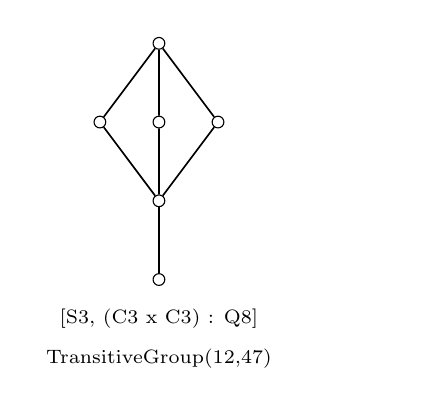
\begin{tikzpicture}[scale=.5]
\matrix[column sep=5mm,row sep=5mm]
{
\node (0) at (0,0) [draw, circle,inner sep=1.5pt] {};
\node (1) at (-0,1) [draw, circle, inner sep=1.5pt] {};
\node (2) at (-0,2) [draw, circle, inner sep=1.5pt] {};
\node (3) at (0.75,2) [draw, circle, inner sep=1.5pt] {};
\node (4) at (-0.75,2) [draw, circle, inner sep=1.5pt] {};
\node (5) at (-0,3) [draw, circle, inner sep=1.5pt] {};
\draw[font=\scriptsize] (0,-.5) node {[S3, (C3 x C3) : Q8]};
\draw[font=\scriptsize] (0,-1) node {TransitiveGroup(12,47) };

\draw[semithick]
(0) to (1)
(1) to (2)
(1) to (3)
(1) to (4)
(2) to (5)
(3) to (5)
(4) to (5);
&
& & \\
};
\end{tikzpicture}
\end{center}
\end{figure}

\newpage


%% \input{TransitiveGsetCongEx14.tex}
\begin{figure}[h]
\caption{Transitive G-set congruence lattices in Eq(14)}
\label{fig:14}
\begin{center}
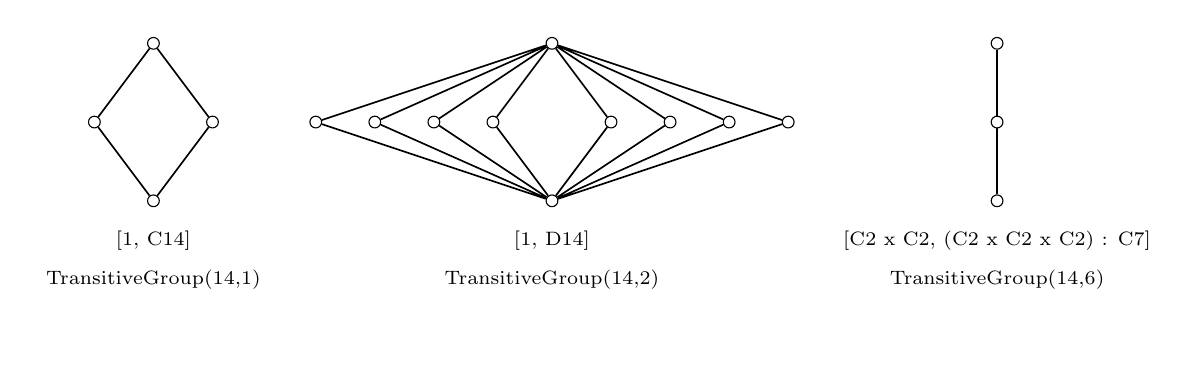
\begin{tikzpicture}[scale=.5]
\matrix[column sep=5mm,row sep=5mm]
{
\node (0) at (0,0) [draw, circle,inner sep=1.5pt] {};
\node (1) at (0.75,1) [draw, circle, inner sep=1.5pt] {};
\node (2) at (-0.75,1) [draw, circle, inner sep=1.5pt] {};
\node (3) at (-0,2) [draw, circle, inner sep=1.5pt] {};
\draw[font=\scriptsize] (0,-.5) node {[1, C14]};
\draw[font=\scriptsize] (0,-1) node {TransitiveGroup(14,1) };

\draw[semithick]
(0) to (1)
(0) to (2)
(1) to (3)
(2) to (3);
&
\node (0) at (0,0) [draw, circle,inner sep=1.5pt] {};
\node (1) at (0.75,1) [draw, circle, inner sep=1.5pt] {};
\node (2) at (-0.75,1) [draw, circle, inner sep=1.5pt] {};
\node (3) at (1.5,1) [draw, circle, inner sep=1.5pt] {};
\node (4) at (-1.5,1) [draw, circle, inner sep=1.5pt] {};
\node (5) at (2.25,1) [draw, circle, inner sep=1.5pt] {};
\node (6) at (-2.25,1) [draw, circle, inner sep=1.5pt] {};
\node (7) at (3,1) [draw, circle, inner sep=1.5pt] {};
\node (8) at (-3,1) [draw, circle, inner sep=1.5pt] {};
\node (9) at (-0,2) [draw, circle, inner sep=1.5pt] {};
\draw[font=\scriptsize] (0,-.5) node {[1, D14]};
\draw[font=\scriptsize] (0,-1) node {TransitiveGroup(14,2) };

\draw[semithick]
(0) to (1)
(0) to (2)
(0) to (3)
(0) to (4)
(0) to (5)
(0) to (6)
(0) to (7)
(0) to (8)
(1) to (9)
(2) to (9)
(3) to (9)
(4) to (9)
(5) to (9)
(6) to (9)
(7) to (9)
(8) to (9);
&
\node (0) at (0,0) [draw, circle,inner sep=1.5pt] {};
\node (1) at (-0,1) [draw, circle, inner sep=1.5pt] {};
\node (2) at (-0,2) [draw, circle, inner sep=1.5pt] {};
\draw[font=\scriptsize] (0,-.5) node {[C2 x C2, (C2 x C2 x C2) : C7]};
\draw[font=\scriptsize] (0,-1) node {TransitiveGroup(14,6) };

\draw[semithick]
(0) to (1)
(1) to (2);
\\
\\
};
\end{tikzpicture}
\end{center}
\end{figure}

\newpage


%% \input{TransitiveGsetCongEx15.tex}
\begin{figure}[h]
\caption{Transitive G-set congruence lattices in Eq(15)}
\label{fig:15}
\begin{center}
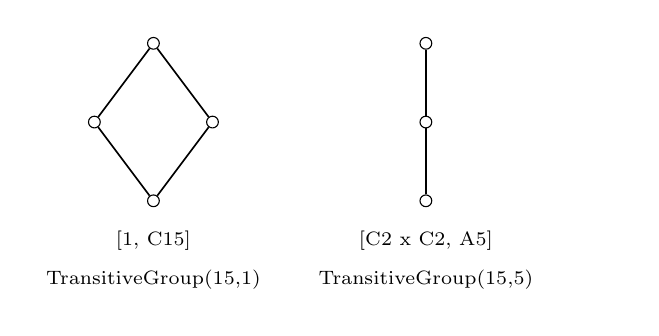
\begin{tikzpicture}[scale=.5]
\matrix[column sep=5mm,row sep=5mm]
{
\node (0) at (0,0) [draw, circle,inner sep=1.5pt] {};
\node (1) at (0.75,1) [draw, circle, inner sep=1.5pt] {};
\node (2) at (-0.75,1) [draw, circle, inner sep=1.5pt] {};
\node (3) at (-0,2) [draw, circle, inner sep=1.5pt] {};
\draw[font=\scriptsize] (0,-.5) node {[1, C15]};
\draw[font=\scriptsize] (0,-1) node {TransitiveGroup(15,1) };

\draw[semithick]
(0) to (1)
(0) to (2)
(1) to (3)
(2) to (3);
&
\node (0) at (0,0) [draw, circle,inner sep=1.5pt] {};
\node (1) at (-0,1) [draw, circle, inner sep=1.5pt] {};
\node (2) at (-0,2) [draw, circle, inner sep=1.5pt] {};
\draw[font=\scriptsize] (0,-.5) node {[C2 x C2, A5]};
\draw[font=\scriptsize] (0,-1) node {TransitiveGroup(15,5) };

\draw[semithick]
(0) to (1)
(1) to (2);
&
& \\
};
\end{tikzpicture}
\end{center}
\end{figure}

\newpage


%\input{TransitiveGsetCongEx16.tex}
%% \input{TransitiveGsetCongEx16CorefreeMin3Max10.tex}
\begin{figure}[h]
\caption{Transitive G-set congruence lattices in Eq(16)}
\label{fig:16}
\begin{center}
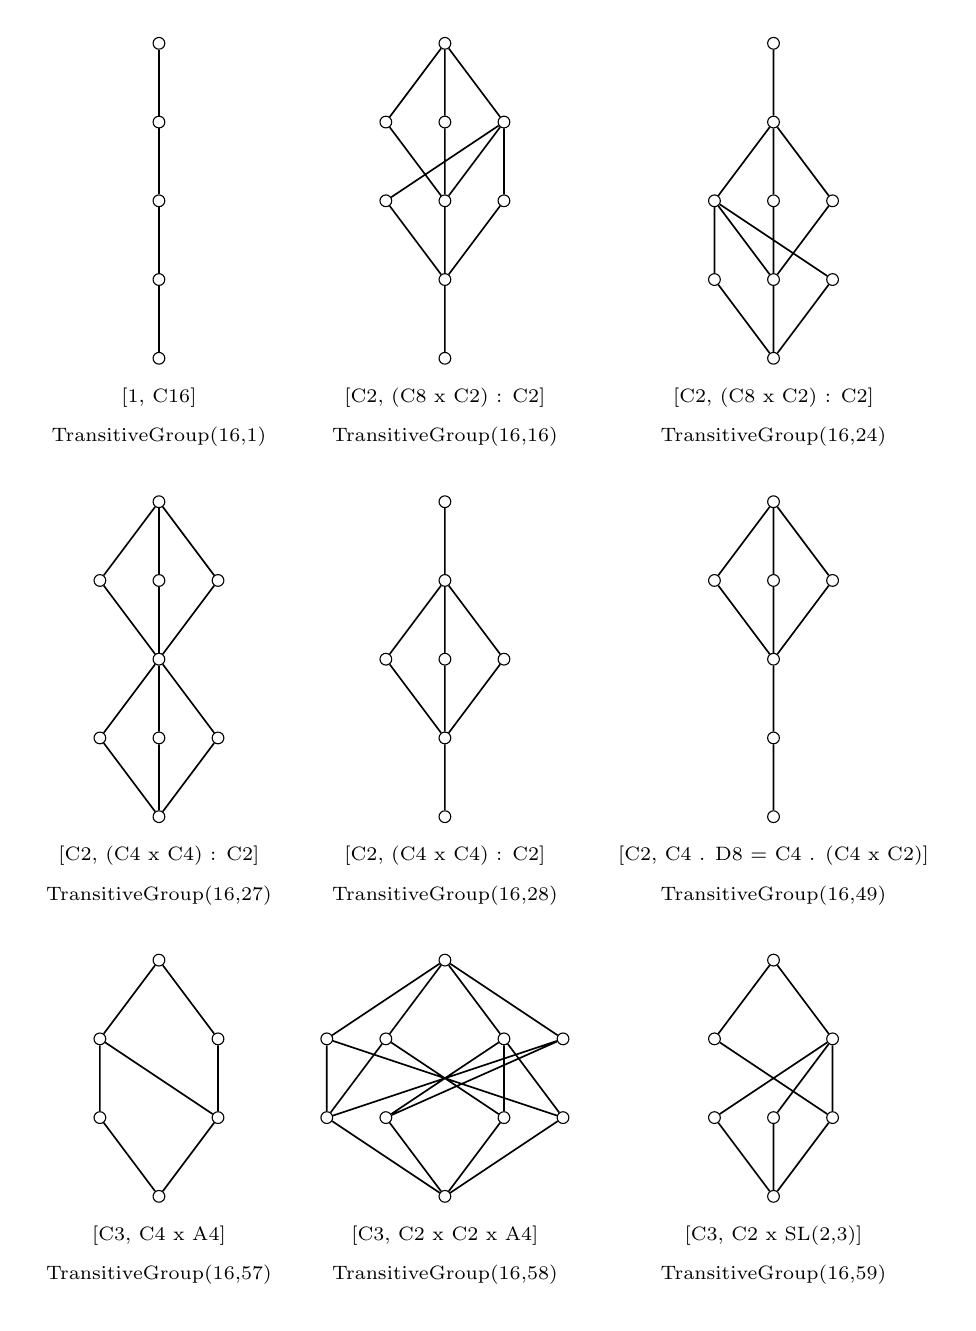
\begin{tikzpicture}[scale=.5]
\matrix[column sep=5mm,row sep=5mm]
{
\node (0) at (0,0) [draw, circle,inner sep=1.5pt] {};
\node (1) at (-0,1) [draw, circle, inner sep=1.5pt] {};
\node (2) at (-0,2) [draw, circle, inner sep=1.5pt] {};
\node (3) at (-0,3) [draw, circle, inner sep=1.5pt] {};
\node (4) at (-0,4) [draw, circle, inner sep=1.5pt] {};
\draw[font=\scriptsize] (0,-.5) node {[1, C16]};
\draw[font=\scriptsize] (0,-1) node {TransitiveGroup(16,1) };

\draw[semithick]
(0) to (1)
(1) to (2)
(2) to (3)
(3) to (4);
&
\node (0) at (0,0) [draw, circle,inner sep=1.5pt] {};
\node (1) at (-0,1) [draw, circle, inner sep=1.5pt] {};
\node (2) at (-0,2) [draw, circle, inner sep=1.5pt] {};
\node (3) at (0.75,2) [draw, circle, inner sep=1.5pt] {};
\node (4) at (-0.75,2) [draw, circle, inner sep=1.5pt] {};
\node (5) at (-0,3) [draw, circle, inner sep=1.5pt] {};
\node (6) at (0.75,3) [draw, circle, inner sep=1.5pt] {};
\node (7) at (-0.75,3) [draw, circle, inner sep=1.5pt] {};
\node (8) at (-0,4) [draw, circle, inner sep=1.5pt] {};
\draw[font=\scriptsize] (0,-.5) node {[C2, (C8 x C2) : C2]};
\draw[font=\scriptsize] (0,-1) node {TransitiveGroup(16,16) };

\draw[semithick]
(0) to (1)
(1) to (2)
(1) to (3)
(1) to (4)
(2) to (5)
(2) to (6)
(2) to (7)
(3) to (6)
(4) to (6)
(5) to (8)
(6) to (8)
(7) to (8);
&
\node (0) at (0,0) [draw, circle,inner sep=1.5pt] {};
\node (1) at (-0,1) [draw, circle, inner sep=1.5pt] {};
\node (2) at (0.75,1) [draw, circle, inner sep=1.5pt] {};
\node (3) at (-0.75,1) [draw, circle, inner sep=1.5pt] {};
\node (4) at (-0,2) [draw, circle, inner sep=1.5pt] {};
\node (5) at (0.75,2) [draw, circle, inner sep=1.5pt] {};
\node (6) at (-0.75,2) [draw, circle, inner sep=1.5pt] {};
\node (7) at (-0,3) [draw, circle, inner sep=1.5pt] {};
\node (8) at (-0,4) [draw, circle, inner sep=1.5pt] {};
\draw[font=\scriptsize] (0,-.5) node {[C2, (C8 x C2) : C2]};
\draw[font=\scriptsize] (0,-1) node {TransitiveGroup(16,24) };

\draw[semithick]
(0) to (1)
(0) to (2)
(0) to (3)
(1) to (4)
(1) to (5)
(1) to (6)
(2) to (6)
(3) to (6)
(4) to (7)
(5) to (7)
(6) to (7)
(7) to (8);
\\
\node (0) at (0,0) [draw, circle,inner sep=1.5pt] {};
\node (1) at (-0,1) [draw, circle, inner sep=1.5pt] {};
\node (2) at (0.75,1) [draw, circle, inner sep=1.5pt] {};
\node (3) at (-0.75,1) [draw, circle, inner sep=1.5pt] {};
\node (4) at (-0,2) [draw, circle, inner sep=1.5pt] {};
\node (5) at (-0,3) [draw, circle, inner sep=1.5pt] {};
\node (6) at (0.75,3) [draw, circle, inner sep=1.5pt] {};
\node (7) at (-0.75,3) [draw, circle, inner sep=1.5pt] {};
\node (8) at (-0,4) [draw, circle, inner sep=1.5pt] {};
\draw[font=\scriptsize] (0,-.5) node {[C2, (C4 x C4) : C2]};
\draw[font=\scriptsize] (0,-1) node {TransitiveGroup(16,27) };

\draw[semithick]
(0) to (1)
(0) to (2)
(0) to (3)
(1) to (4)
(2) to (4)
(3) to (4)
(4) to (5)
(4) to (6)
(4) to (7)
(5) to (8)
(6) to (8)
(7) to (8);
&
\node (0) at (0,0) [draw, circle,inner sep=1.5pt] {};
\node (1) at (-0,1) [draw, circle, inner sep=1.5pt] {};
\node (2) at (-0,2) [draw, circle, inner sep=1.5pt] {};
\node (3) at (0.75,2) [draw, circle, inner sep=1.5pt] {};
\node (4) at (-0.75,2) [draw, circle, inner sep=1.5pt] {};
\node (5) at (-0,3) [draw, circle, inner sep=1.5pt] {};
\node (6) at (-0,4) [draw, circle, inner sep=1.5pt] {};
\draw[font=\scriptsize] (0,-.5) node {[C2, (C4 x C4) : C2]};
\draw[font=\scriptsize] (0,-1) node {TransitiveGroup(16,28) };

\draw[semithick]
(0) to (1)
(1) to (2)
(1) to (3)
(1) to (4)
(2) to (5)
(3) to (5)
(4) to (5)
(5) to (6);
&
\node (0) at (0,0) [draw, circle,inner sep=1.5pt] {};
\node (1) at (-0,1) [draw, circle, inner sep=1.5pt] {};
\node (2) at (-0,2) [draw, circle, inner sep=1.5pt] {};
\node (3) at (-0,3) [draw, circle, inner sep=1.5pt] {};
\node (4) at (0.75,3) [draw, circle, inner sep=1.5pt] {};
\node (5) at (-0.75,3) [draw, circle, inner sep=1.5pt] {};
\node (6) at (-0,4) [draw, circle, inner sep=1.5pt] {};
\draw[font=\scriptsize] (0,-.5) node {[C2, C4 . D8 = C4 . (C4 x C2)]};
\draw[font=\scriptsize] (0,-1) node {TransitiveGroup(16,49) };

\draw[semithick]
(0) to (1)
(1) to (2)
(2) to (3)
(2) to (4)
(2) to (5)
(3) to (6)
(4) to (6)
(5) to (6);
\\
\node (0) at (0,0) [draw, circle,inner sep=1.5pt] {};
\node (1) at (0.75,1) [draw, circle, inner sep=1.5pt] {};
\node (2) at (0.75,2) [draw, circle, inner sep=1.5pt] {};
\node (3) at (-0.75,1) [draw, circle, inner sep=1.5pt] {};
\node (4) at (-0.75,2) [draw, circle, inner sep=1.5pt] {};
\node (5) at (-0,3) [draw, circle, inner sep=1.5pt] {};
\draw[font=\scriptsize] (0,-.5) node {[C3, C4 x A4]};
\draw[font=\scriptsize] (0,-1) node {TransitiveGroup(16,57) };

\draw[semithick]
(0) to (1)
(0) to (3)
(1) to (2)
(1) to (4)
(2) to (5)
(3) to (4)
(4) to (5);
&
\node (0) at (0,0) [draw, circle,inner sep=1.5pt] {};
\node (1) at (0.75,1) [draw, circle, inner sep=1.5pt] {};
\node (2) at (-0.75,1) [draw, circle, inner sep=1.5pt] {};
\node (3) at (1.5,1) [draw, circle, inner sep=1.5pt] {};
\node (4) at (-1.5,1) [draw, circle, inner sep=1.5pt] {};
\node (5) at (0.75,2) [draw, circle, inner sep=1.5pt] {};
\node (6) at (-0.75,2) [draw, circle, inner sep=1.5pt] {};
\node (7) at (1.5,2) [draw, circle, inner sep=1.5pt] {};
\node (8) at (-1.5,2) [draw, circle, inner sep=1.5pt] {};
\node (9) at (-0,3) [draw, circle, inner sep=1.5pt] {};
\draw[font=\scriptsize] (0,-.5) node {[C3, C2 x C2 x A4]};
\draw[font=\scriptsize] (0,-1) node {TransitiveGroup(16,58) };

\draw[semithick]
(0) to (1)
(0) to (2)
(0) to (3)
(0) to (4)
(1) to (5)
(1) to (6)
(2) to (5)
(2) to (7)
(3) to (5)
(3) to (8)
(4) to (6)
(4) to (7)
(4) to (8)
(5) to (9)
(6) to (9)
(7) to (9)
(8) to (9);
&
\node (0) at (0,0) [draw, circle,inner sep=1.5pt] {};
\node (1) at (-0,1) [draw, circle, inner sep=1.5pt] {};
\node (2) at (0.75,1) [draw, circle, inner sep=1.5pt] {};
\node (3) at (-0.75,1) [draw, circle, inner sep=1.5pt] {};
\node (4) at (0.75,2) [draw, circle, inner sep=1.5pt] {};
\node (5) at (-0.75,2) [draw, circle, inner sep=1.5pt] {};
\node (6) at (-0,3) [draw, circle, inner sep=1.5pt] {};
\draw[font=\scriptsize] (0,-.5) node {[C3, C2 x SL(2,3)]};
\draw[font=\scriptsize] (0,-1) node {TransitiveGroup(16,59) };

\draw[semithick]
(0) to (1)
(0) to (2)
(0) to (3)
(1) to (4)
(2) to (4)
(2) to (5)
(3) to (4)
(4) to (6)
(5) to (6);
\\
};
\end{tikzpicture}
\end{center}
\end{figure}

\newpage

\begin{figure}[h]
\caption{Transitive G-set congruence lattices in Eq(16) (continued)}
\label{fig:16b}
\begin{center}
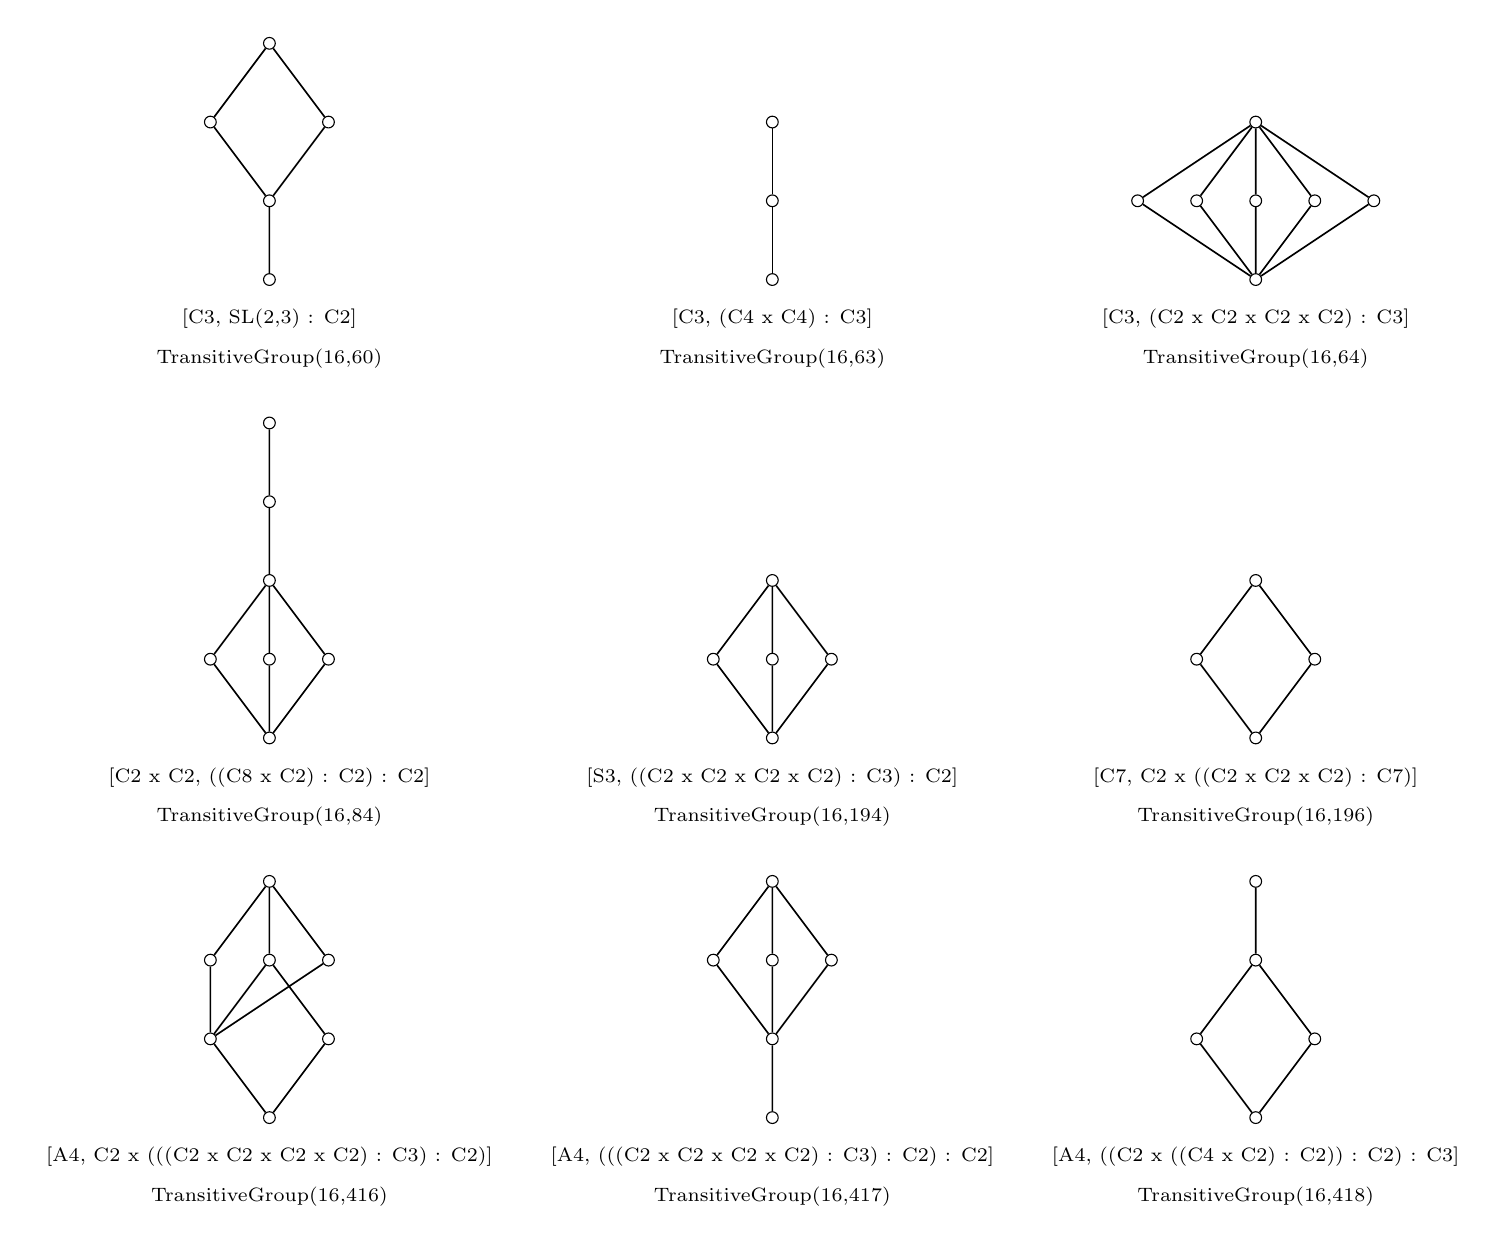
\begin{tikzpicture}[scale=.5]
\matrix[column sep=5mm,row sep=5mm]
{
\node (0) at (0,0) [draw, circle,inner sep=1.5pt] {};
\node (1) at (-0,1) [draw, circle, inner sep=1.5pt] {};
\node (2) at (0.75,2) [draw, circle, inner sep=1.5pt] {};
\node (3) at (-0.75,2) [draw, circle, inner sep=1.5pt] {};
\node (4) at (-0,3) [draw, circle, inner sep=1.5pt] {};
\draw[font=\scriptsize] (0,-.5) node {[C3, SL(2,3) : C2]};
\draw[font=\scriptsize] (0,-1) node {TransitiveGroup(16,60) };

\draw[semithick]
(0) to (1)
(1) to (2)
(1) to (3)
(2) to (4)
(3) to (4);
&
\node (0) at (0,0) [draw, circle,inner sep=1.5pt] {};
\node (1) at (-0,1) [draw, circle, inner sep=1.5pt] {};
\node (2) at (-0,2) [draw, circle, inner sep=1.5pt] {};
\draw[font=\scriptsize] (0,-.5) node {[C3, (C4 x C4) : C3]};
\draw[font=\scriptsize] (0,-1) node {TransitiveGroup(16,63) };

\draw[semithick]
(0) to (1)
(1) to (2);
&
\node (0) at (0,0) [draw, circle,inner sep=1.5pt] {};
\node (1) at (-0,1) [draw, circle, inner sep=1.5pt] {};
\node (2) at (0.75,1) [draw, circle, inner sep=1.5pt] {};
\node (3) at (-0.75,1) [draw, circle, inner sep=1.5pt] {};
\node (4) at (1.5,1) [draw, circle, inner sep=1.5pt] {};
\node (5) at (-1.5,1) [draw, circle, inner sep=1.5pt] {};
\node (6) at (-0,2) [draw, circle, inner sep=1.5pt] {};
\draw[font=\scriptsize] (0,-.5) node {[C3, (C2 x C2 x C2 x C2) : C3]};
\draw[font=\scriptsize] (0,-1) node {TransitiveGroup(16,64) };

\draw[semithick]
(0) to (1)
(0) to (2)
(0) to (3)
(0) to (4)
(0) to (5)
(1) to (6)
(2) to (6)
(3) to (6)
(4) to (6)
(5) to (6);
\\
\node (0) at (0,0) [draw, circle,inner sep=1.5pt] {};
\node (1) at (-0,1) [draw, circle, inner sep=1.5pt] {};
\node (2) at (0.75,1) [draw, circle, inner sep=1.5pt] {};
\node (3) at (-0.75,1) [draw, circle, inner sep=1.5pt] {};
\node (4) at (-0,2) [draw, circle, inner sep=1.5pt] {};
\node (5) at (-0,3) [draw, circle, inner sep=1.5pt] {};
\node (6) at (-0,4) [draw, circle, inner sep=1.5pt] {};
\draw[font=\scriptsize] (0,-.5) node {[C2 x C2, ((C8 x C2) : C2) : C2]};
\draw[font=\scriptsize] (0,-1) node {TransitiveGroup(16,84) };

\draw[semithick]
(0) to (1)
(0) to (2)
(0) to (3)
(1) to (4)
(2) to (4)
(3) to (4)
(4) to (5)
(5) to (6);
&
\node (0) at (0,0) [draw, circle,inner sep=1.5pt] {};
\node (1) at (-0,1) [draw, circle, inner sep=1.5pt] {};
\node (2) at (0.75,1) [draw, circle, inner sep=1.5pt] {};
\node (3) at (-0.75,1) [draw, circle, inner sep=1.5pt] {};
\node (4) at (-0,2) [draw, circle, inner sep=1.5pt] {};
\draw[font=\scriptsize] (0,-.5) node {[S3, ((C2 x C2 x C2 x C2) : C3) : C2]};
\draw[font=\scriptsize] (0,-1) node {TransitiveGroup(16,194) };

\draw[semithick]
(0) to (1)
(0) to (2)
(0) to (3)
(1) to (4)
(2) to (4)
(3) to (4);
&
\node (0) at (0,0) [draw, circle,inner sep=1.5pt] {};
\node (1) at (0.75,1) [draw, circle, inner sep=1.5pt] {};
\node (2) at (-0.75,1) [draw, circle, inner sep=1.5pt] {};
\node (3) at (-0,2) [draw, circle, inner sep=1.5pt] {};
\draw[font=\scriptsize] (0,-.5) node {[C7, C2 x ((C2 x C2 x C2) : C7)]};
\draw[font=\scriptsize] (0,-1) node {TransitiveGroup(16,196) };

\draw[semithick]
(0) to (1)
(0) to (2)
(1) to (3)
(2) to (3);
\\
\node (0) at (0,0) [draw, circle,inner sep=1.5pt] {};
\node (1) at (0.75,1) [draw, circle, inner sep=1.5pt] {};
\node (2) at (-0.75,1) [draw, circle, inner sep=1.5pt] {};
\node (3) at (-0,2) [draw, circle, inner sep=1.5pt] {};
\node (4) at (0.75,2) [draw, circle, inner sep=1.5pt] {};
\node (5) at (-0.75,2) [draw, circle, inner sep=1.5pt] {};
\node (6) at (-0,3) [draw, circle, inner sep=1.5pt] {};
\draw[font=\scriptsize] (0,-.5) node {[A4, C2 x (((C2 x C2 x C2 x C2) : C3) : C2)]};
\draw[font=\scriptsize] (0,-1) node {TransitiveGroup(16,416) };

\draw[semithick]
(0) to (1)
(0) to (2)
(1) to (3)
(2) to (3)
(2) to (4)
(2) to (5)
(3) to (6)
(4) to (6)
(5) to (6);
&
\node (0) at (0,0) [draw, circle,inner sep=1.5pt] {};
\node (1) at (-0,1) [draw, circle, inner sep=1.5pt] {};
\node (2) at (-0,2) [draw, circle, inner sep=1.5pt] {};
\node (3) at (0.75,2) [draw, circle, inner sep=1.5pt] {};
\node (4) at (-0.75,2) [draw, circle, inner sep=1.5pt] {};
\node (5) at (-0,3) [draw, circle, inner sep=1.5pt] {};
\draw[font=\scriptsize] (0,-.5) node {[A4, (((C2 x C2 x C2 x C2) : C3) : C2) : C2]};
\draw[font=\scriptsize] (0,-1) node {TransitiveGroup(16,417) };

\draw[semithick]
(0) to (1)
(1) to (2)
(1) to (3)
(1) to (4)
(2) to (5)
(3) to (5)
(4) to (5);
&
\node (0) at (0,0) [draw, circle,inner sep=1.5pt] {};
\node (1) at (0.75,1) [draw, circle, inner sep=1.5pt] {};
\node (2) at (-0.75,1) [draw, circle, inner sep=1.5pt] {};
\node (3) at (-0,2) [draw, circle, inner sep=1.5pt] {};
\node (4) at (-0,3) [draw, circle, inner sep=1.5pt] {};
\draw[font=\scriptsize] (0,-.5) node {[A4, ((C2 x ((C4 x C2) : C2)) : C2) : C3]};
\draw[font=\scriptsize] (0,-1) node {TransitiveGroup(16,418) };

\draw[semithick]
(0) to (1)
(0) to (2)
(1) to (3)
(2) to (3)
(3) to (4);
\\
};
\end{tikzpicture}
\end{center}
\end{figure}

\newpage

\begin{figure}[h]
\caption{Transitive G-set congruence lattices in Eq(16) (continued)}
\label{fig:16c}
\begin{center}
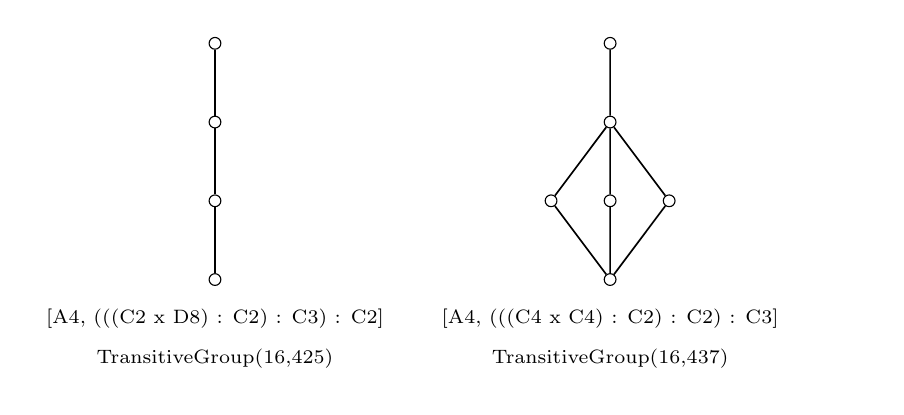
\begin{tikzpicture}[scale=.5]
\matrix[column sep=5mm,row sep=5mm]
{
\node (0) at (0,0) [draw, circle,inner sep=1.5pt] {};
\node (1) at (-0,1) [draw, circle, inner sep=1.5pt] {};
\node (2) at (-0,2) [draw, circle, inner sep=1.5pt] {};
\node (3) at (-0,3) [draw, circle, inner sep=1.5pt] {};
\draw[font=\scriptsize] (0,-.5) node {[A4, (((C2 x D8) : C2) : C3) : C2]};
\draw[font=\scriptsize] (0,-1) node {TransitiveGroup(16,425) };

\draw[semithick]
(0) to (1)
(1) to (2)
(2) to (3);
&
\node (0) at (0,0) [draw, circle,inner sep=1.5pt] {};
\node (1) at (-0,1) [draw, circle, inner sep=1.5pt] {};
\node (2) at (0.75,1) [draw, circle, inner sep=1.5pt] {};
\node (3) at (-0.75,1) [draw, circle, inner sep=1.5pt] {};
\node (4) at (-0,2) [draw, circle, inner sep=1.5pt] {};
\node (5) at (-0,3) [draw, circle, inner sep=1.5pt] {};
\draw[font=\scriptsize] (0,-.5) node {[A4, (((C4 x C4) : C2) : C2) : C3]};
\draw[font=\scriptsize] (0,-1) node {TransitiveGroup(16,437) };

\draw[semithick]
(0) to (1)
(0) to (2)
(0) to (3)
(1) to (4)
(2) to (4)
(3) to (4)
(4) to (5);
&
& \\
};
\end{tikzpicture}
\end{center}
\end{figure}

\newpage


%\input{TransitiveGsetCongEx16CorefreeMin3Max14.tex}

